\documentclass[12pt, a4paper, oneside]{ctexart}
\usepackage{amsmath, amsthm, amssymb, bm, color, graphicx, geometry, hyperref, mathrsfs,extarrows, braket}

\linespread{1.5}
\geometry{left=2.54cm,right=2.54cm,top=3.18cm,bottom=3.18cm}
\newenvironment{problem}{\par\noindent\textbf{题目. }}{\bigskip\par}
\newenvironment{solution}{\par\noindent\textbf{解答. }}{\bigskip\par}
\newenvironment{note}{\par\noindent\textbf{注记. }}{\bigskip\par}

% 基本信息
\newcommand{\dt}{\today}
\newcommand{\sj}{离散数学}
\newcommand{\vt}{吴天阳 2204210460}

\begin{document}

\pagestyle{empty}
\vspace*{-20ex}
\centerline{\begin{tabular}{*3{c}}
    \parbox[t]{0.3\linewidth}{\begin{center}\textbf{日期}\\ \large \textcolor{blue}{\dt}\end{center}} 
    & \parbox[t]{0.3\linewidth}{\begin{center}\textbf{科目}\\ \large \textcolor{blue}{\sj}\end{center}}
    & \parbox[t]{0.3\linewidth}{\begin{center}\textbf{姓名,学号}\\ \large \textcolor{blue}{\vt}\end{center}} \\ \hline
\end{tabular}}
\vspace*{4ex}
\paragraph{习题八}
\paragraph{16.}\begin{solution}
    如图所示:

    \centerline{
        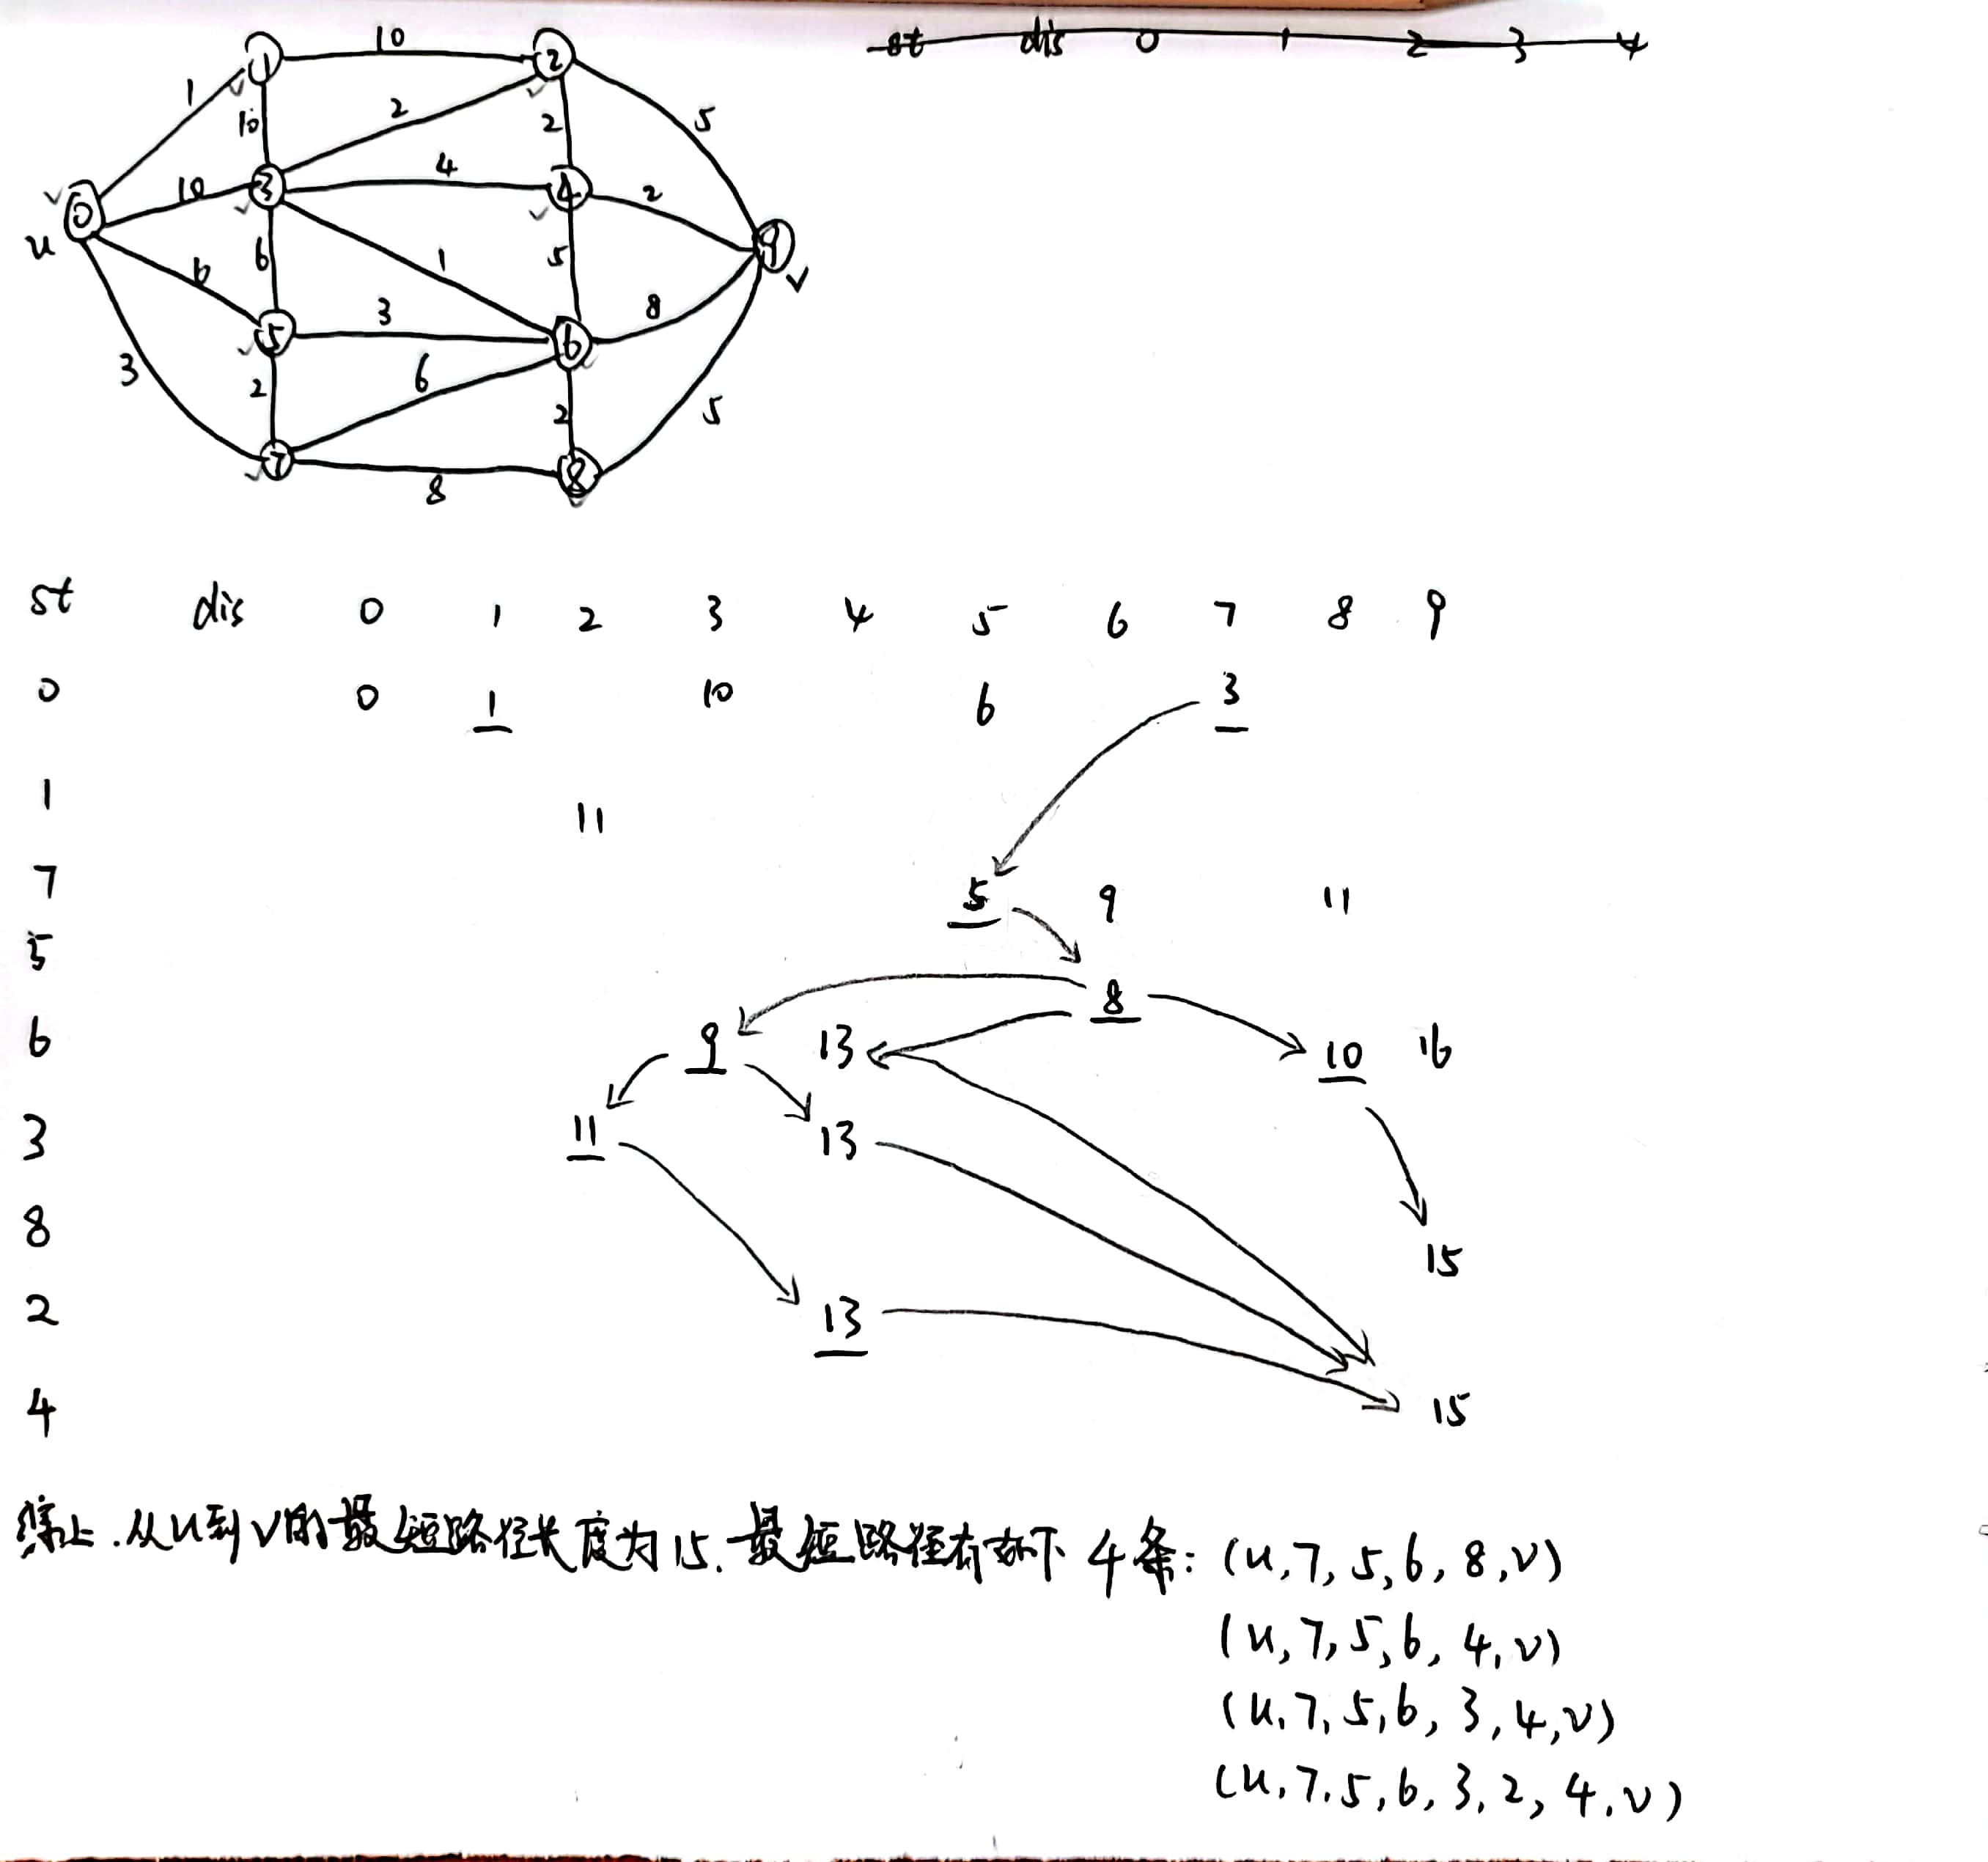
\includegraphics[width=1\textwidth]{graph.jpg}
    }
\end{solution}
\newpage
\paragraph{20.}\begin{proof}
    由于图中奇结点的个数一定为偶数个,设一个连通图中奇结点个数为$n=2k>0$,使用以下方法将$G$中的边划分为多条不交的简单路,考虑以下两种情况:

    1. 如果该图$G_i$中$k=1$,则存在$Euler$路$C_i$使得$E(C_i) = E(G_i)$。

    2. 如果该图$G_i$中$k\geqslant 2$,则任取图中两个在同一个连通图中的奇结点分别记为$u,v$,由$G_i$的连通性知,至少存在一条以$u,v$作为起终结点的路径$C_i$,将$G_i$中所有$C_i$中的边去掉变为$G_{i+1}$,则$G_{i+1}$中的奇结点个数为$2(k-1)$,因为去掉$C_i$中的边,只会导致$u,v$的度数减一(奇偶性改变,均变为偶结点),其他中间结点的度数减二(奇偶性不变)。

    如果连通图$G$的奇结点个数为$2k$,若$k$大于$1$,可通过方法2减少奇结点的个数,最终化为方法1,则至多减去$k$条路径,分别记为$C_1,C_2,\cdots,C_k$,由于
    \begin{equation*}
        \begin{aligned}
            &G = G_1\\
            &E(G_i) = E(G_{i+1})\cup E(C_i)&(i=1,2,\cdots,k-1)\\
            &E(G_k) = E(C_k)
        \end{aligned}
    \end{equation*}
    又由于每次路径中的边都被去掉,所以所选的路径的边互不相交,且
    \begin{equation*}
        E(G) = \bigcup_{i=1}^kE(C_i)
    \end{equation*}
\end{proof}

\end{document}
